% ACIIDS 2027 submission (Springer LNCS/LNAI template, as required by the conference).
\documentclass[runningheads]{llncs}
\usepackage[T1]{fontenc}
\usepackage{graphicx}
\usepackage{amsmath,amssymb}
\usepackage{booktabs}
\usepackage{array}
\usepackage{xcolor}
\usepackage{algorithm}
\usepackage[noend]{algpseudocode}
\usepackage{tikz}
\usetikzlibrary{positioning,arrows.meta}
\usepackage[hidelinks]{hyperref}
\newcommand{\duet}{\mbox{DUET}}\newcommand{\duetD}{\mbox{DUET-D}}\newcommand{\duetE}{\mbox{DUET-E}}
\newcommand{\bts}{\mbox{DUET-M}}
\newcommand{\Hd}{H_{\mathrm{d}}}
\renewcommand{\topfraction}{0.9}\renewcommand{\bottomfraction}{0.8}\renewcommand{\textfraction}{0.07}\renewcommand{\floatpagefraction}{0.85}\setcounter{topnumber}{3}\setcounter{totalnumber}{4}
\renewcommand{\algorithmiccomment}[1]{\hfill{\footnotesize$\triangleright$ #1}}

\begin{document}
\setlength{\emergencystretch}{1.5em}
\title{DUET: Efficient Pairwise Search for Electromagnetically Coupled Meta-Atoms in Reconfigurable Intelligent Surfaces}
\titlerunning{DUET: Pairwise Search for Coupled RIS Meta-Atoms}
\author{Muhammad Faris El~Hakim \and Ahmad Dzaki Hakiim~Fadhlurrohman \and Widhi~Yahya}
\authorrunning{M. F. El Hakim et al.}
\institute{Universitas Brawijaya, Malang, Indonesia\\
\email{fariselhakim898@gmail.com, ahmaddzaki195@gmail.com, widhi.yahya@ub.ac.id}}
\maketitle

\begin{abstract}
Configuring a 1-bit reconfigurable intelligent surface (RIS) to maximise the minimum user rate is a binary max--min problem that must be re-solved within tens of milliseconds as users move. Evolutionary controllers such as ME-GA and NSGA-II are commonly applied to this problem; however, when mutual coupling between elements is modelled, every candidate configuration requires a separate evaluation of the coupled multiport network. This paper proposes DUET, a deadline-bounded pairwise local search that evaluates every single-element and two-element flip exactly through rank-one and rank-two updates of the coupled network, together with \bts{}, a variant that adds restart densities and elite recombination. All methods share the same evaluator, the same CPU core and a hard deadline that includes evaluator set-up. On the sealed Rotterdam test split of GeoRIS-Bench, which combines LoD2 city models, ray tracing and a method-of-moments surface model, \bts{} exceeds ME-GA by 0.23 and 0.77\,bit/s/Hz and NSGA-II by 0.06 and 0.45\,bit/s/Hz for 64- and 128-element surfaces under a 50\,ms deadline, since pair moves evaluate 62--445 times more candidates in the same time. Plain \duet{} attains the same rates. Without retuning, its gains over both evolutionary baselines are preserved on 72 sealed trajectories from two unseen cities. For 256-element surfaces, a single exhaustive pair scan exceeds the time reserved for it, which identifies scan scheduling under hard deadlines as an open problem.
\keywords{Reconfigurable intelligent surface \and Combinatorial optimisation \and Anytime search \and Local search \and Evolutionary algorithms \and Mutual coupling.}
\end{abstract}

%======================================================================
\section{Introduction}
%======================================================================
A reconfigurable intelligent surface (RIS) is a passive array whose elements switch between a small number of load states, so that the re-radiated field can be shaped without active transmit chains~\cite{li2026tutorial}. With 1-bit elements, configuring an $N$-element surface amounts to selecting one of $2^N$ binary states. When the surface assists a multi-antenna base station (BS) that serves several users, a common fairness objective is the rate of the worst-served user. This objective is non-smooth and, once mutual coupling between elements is modelled~\cite{qian2021mutual,zheng2024mutual,nerini2024universal,nerini2026global}, also non-separable, because the contribution of each element depends on the states of all others. As users move, the configuration must be recomputed every few tens of milliseconds on the surface controller~\cite{urbinati2026ondevice}. The relevant question is therefore not which method attains the global optimum, but which method returns the best configuration \emph{within a fixed deadline}.

Evolutionary algorithms are widely used in this setting~\cite{stylianopoulos2022dlga,zardi2024memory}. Zardi, Oliveri and Massa~\cite{zardi2024memory} proposed ME-GA, a genetic algorithm that maintains a memory of earlier high-quality individuals in order to track a time-varying channel, and NSGA-II~\cite{deb2002fast} remains the standard elitist evolutionary algorithm. Under a deadline, however, their limiting factor is evaluation cost: unless an individual is close to an already evaluated state, it requires a linear solve with the $N\times N$ impedance matrix of the coupled network. Single-flip local search is considerably cheaper, since a flip changes one diagonal load and can be evaluated by a rank-one update, but it terminates prematurely: a configuration may be optimal with respect to every single flip and still be improvable by flipping two coupled elements jointly.

This paper therefore builds \duet{} (Deadline-bounded Updates for Exact Two-flip search) on exact pair moves. Pair flips, restarts, elite recombination and low-rank updates are individually well established~\cite{merz2002bqp,lourenco2010ils,merz2004memetic,prodhomme2023efficient}; to the best of our knowledge, however, existing RIS configuration studies are limited to single-flip descent~\cite{hammami2026statistical}. The contributions of this paper are as follows:
\begin{enumerate}
\item \textbf{\duet{}, a deadline-bounded exact pair-neighbourhood search} for coupled 1-bit RIS control under a non-quadratic multiuser max--min rate objective. All $N$ single flips and all $N(N-1)/2$ pair flips are evaluated exactly by rank-one and rank-two updates of the coupled network; the variant \bts{} adds two pre-declared restart densities and elite recombination, forming a memetic iterated local search (Sect.~\ref{sec:method}).
\item \textbf{A deadline-fair evaluation protocol} in which all methods share one evaluator, one deadline that includes set-up, and three metrics (worst-user spectral efficiency, latency, budget), with decision rules fixed before the held-out evaluation (Sect.~\ref{sec:protocol}).
\item \textbf{An evaluation on three European cities} of GeoRIS-Bench~\cite{georisbench} (Rotterdam and two held-out cities) against single-flip search, ME-GA and NSGA-II at 64--256 elements, with an analysis of why exhaustive pair scans cease to meet the deadline at 256 elements (Sects.~\ref{sec:results} and~\ref{sec:discussion}).
\end{enumerate}

%======================================================================
\section{Related Work}\label{sec:related}
%======================================================================
Table~\ref{tab:related} groups prior RIS configuration methods into six families and summarises the limitation of each with respect to the setting considered here: a mutually coupled 1-bit surface, a multiuser max--min objective and a hard decision-time deadline.

\begin{table}[t]
\centering
\caption{Families of RIS configuration methods and their limitations for deadline-bounded control of a coupled 1-bit surface.}\label{tab:related}
\scriptsize\setlength{\tabcolsep}{3pt}\renewcommand{\arraystretch}{1.05}
\begin{tabular}{@{}>{\raggedright\arraybackslash}p{0.14\textwidth}>{\raggedright\arraybackslash}p{0.16\textwidth}>{\raggedright\arraybackslash}p{0.35\textwidth}>{\raggedright\arraybackslash}p{0.29\textwidth}@{}}
\toprule
Family & Works & Approach & Limitation for this setting\\
\midrule
Direct learned prediction & \cite{martin2024hardware,padial2026accelerating,urbinati2026ondevice,xu2022robust} & one-pass network prediction of the configuration; FPGA/MCU latency reported & trained offline per array and task; no search at decision time\\
Physics-aware learning & \cite{peng2025risnet,liu2026physics} & coupling-aware unsupervised network (multiuser SDMA); full-wave surrogate searched by NSGA-II & optimisation amortised into training; not compared with search under a deadline\\
Evolutionary control & \cite{stylianopoulos2022dlga,radar2024onebitga,zardi2024memory} \cite{deb2002fast,lange2023discovering} & population search; ME-GA keeps a memory of past best individuals; learned operators & one coupled evaluation per individual limits the candidates evaluated within a deadline\\
Analytical and coordinate methods & \cite{zhang2022configuring,qian2021mutual,hammami2026statistical,nerini2026global} & optimal binary state for single-user SNR; coordinate descent and closed-form optima with coupling & restricted to single-user, continuous or single-flip settings\\
Coupled-channel computation & \cite{faqiri2023physfad,prodhomme2023efficient} & coupled-dipole models; rank-$m$ channel updates & used for channel computation rather than within a search\\
Binary quadratic local search & \cite{merz2002bqp,lourenco2010ils,merz2004memetic} \cite{glover2010ddts,lu2010hybrid,wang2012pathrelinking} & 1-opt and $k$-opt moves, iterated local search, memetic and path-relinking methods & move gains assume a quadratic objective; the coupled max--min rate is not quadratic\\
\midrule
This paper & -- & exact single and pair moves (rank-one/two updates) within a hard CPU deadline & --\\
\bottomrule
\end{tabular}
\end{table}

The works closest to ours are single-flip (coordinate) descent on multiport RIS models~\cite{hammami2026statistical}, the low-rank channel updates of Prod'homme and del Hougne~\cite{prodhomme2023efficient}, and $k$-opt local search for binary quadratic programmes~\cite{merz2002bqp}. The proposed method combines the latter two: the rank-two update makes the complete pair neighbourhood inexpensive enough to be scanned at every step, which removes the single-flip restriction of the former. The impedance-domain channel model follows multiport network theory~\cite{nerini2024universal,nossek2024physically,abrardo2024design,li2026tutorial}. Measured 5\,GHz datasets, open hardware~\cite{tewes2023comprehensive,rossanese2024open,piana2026brisc,heinrichs2023open} and simulators~\cite{burtakov2023qris} provide channels but do not define a deadline-bounded protocol for comparing configuration methods.

%======================================================================
\section{Problem and Coupled Evaluator}\label{sec:problem}
%======================================================================
\textbf{Channel.} The surface comprises $N$ thin-wire elements, each terminated by one of two passive loads $z_0,z_1$ (1\,$\Omega$ resistance, reactances $\pm70\,\Omega$ around the isolated-wire resonance). Let $Z_{\mathrm{RIS}}$ be the full $N\times N$ impedance matrix from NEC-2~\cite{burke1981nec,pynec}, after a Schur-complement reduction over the 50\,$\Omega$-terminated BS and user ports. With $Z_L(\mathbf b)=\mathrm{diag}(z_{b_1},\dots,z_{b_N})$ and $T(\mathbf b)=(Z_{\mathrm{RIS}}+Z_L(\mathbf b))^{-1}$, the channel from the four BS ports to the $K$ users is
\begin{equation}
H(\mathbf b)=\Hd + C_{\mathrm{out}}\,T(\mathbf b)\,C_{\mathrm{in}},
\label{eq:operator}
\end{equation}
where $\Hd$ is the direct channel and $C_{\mathrm{in}}$, $C_{\mathrm{out}}$ couple the elements to the BS and the users. The off-diagonal entries of $Z_{\mathrm{RIS}}$ represent mutual coupling, which renders the response of each element dependent on the states of all others.

\textbf{Objective.} A regularised zero-forcing precoder $W$ is computed once from the all-OFF channel and kept fixed. With effective field $U(\mathbf b)=H(\mathbf b)W$ and noise power $\sigma^2$,
\begin{equation}
\max_{\mathbf b\in\{0,1\}^N} f(\mathbf b),\qquad f(\mathbf b)=\min_{k}\log_2\Bigl(1+\frac{|U_{kk}|^2}{\sum_{j\ne k}|U_{kj}|^2+\sigma^2}\Bigr).
\label{eq:objective}
\end{equation}

\textbf{Exact single and pair moves.} Flipping element $i$ changes one diagonal load by $\delta_i=z_{1-b_i}-z_{b_i}$. Given $T$, precompute $L=C_{\mathrm{out}}T\in\mathbb C^{K\times N}$, $R=TC_{\mathrm{in}}W\in\mathbb C^{N\times S}$ and $d_i=1/\delta_i+T_{ii}$. By Sherman--Morrison, the field after flipping $i$ is
\begin{equation}
U^{(i)}=U-\frac{\ell_i\,r_i^{\top}}{d_i},
\end{equation}
with $\ell_i$ the $i$-th column of $L$ and $r_i^\top$ the $i$-th row of $R$. For a pair $(i,j)$, the $2\times2$ Woodbury identity gives, with $\Delta_{ij}=d_id_j-T_{ij}T_{ji}$,
\begin{equation}
U^{(ij)}=U-\ell_i u_i^{\top}-\ell_j u_j^{\top},\quad u_i=\frac{d_jr_i-T_{ij}r_j}{\Delta_{ij}},\quad u_j=\frac{d_ir_j-T_{ji}r_i}{\Delta_{ij}}.
\label{eq:pair}
\end{equation}
\textbf{Cost.} Forming $L$ and $R$ costs $O(N^2(K+S))$ once per state. Each single move then costs $O(KS)$ and each pair move $O(KS)$ plus a $2\times2$ determinant, so a full scan of all $N(N-1)/2$ pairs costs $O(N^2KS)$. Scoring each pair by a fresh inverse would cost $O(N^3)$ per candidate, i.e.\ $O(N^5)$ per scan. Committing an accepted move updates $T$ by a rank-one or rank-two correction in $O(N^2)$. All methods in this paper, including the evolutionary baselines, use this evaluator.

%======================================================================
\section{Method}\label{sec:method}
%======================================================================
Figure~\ref{fig:workflow} contrasts \duet{} with the evolutionary baselines. Its variants differ only in the restart rule: \duetD{} (density restarts), \duetE{} (elite recombination) and \bts{} (both, a memetic search).

\begin{figure}[t]
\centering
\resizebox{\textwidth}{!}{%
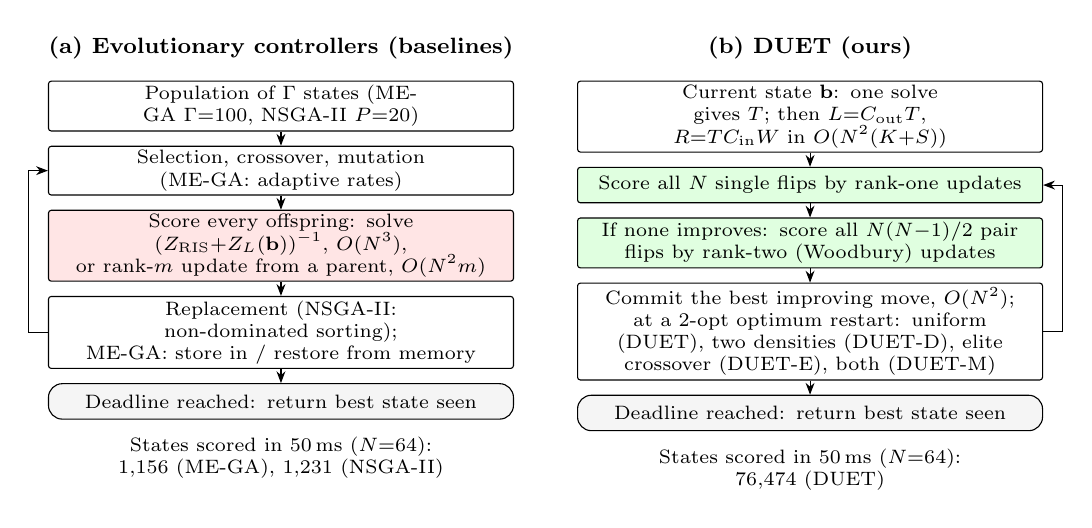
\begin{tikzpicture}[font=\scriptsize, node distance=1.8mm,
 box/.style={draw, rounded corners=1pt, align=center, text width=58mm, inner sep=1.5pt, minimum height=4.5mm},
 slow/.style={box, fill=red!10}, fast/.style={box, fill=green!12},
 stop/.style={box, rounded corners=5pt, fill=gray!8},
 arr/.style={-{Stealth[length=1.5mm]}}]
\node[font=\footnotesize\bfseries, align=center] (ta) {(a) Evolutionary controllers (baselines)};
\node[box, below=1.5mm of ta] (a1) {Population of $\Gamma$ states (ME-GA $\Gamma{=}100$, NSGA-II $P{=}20$)};
\node[box, below=of a1] (a2) {Selection, crossover, mutation\\(ME-GA: adaptive rates)};
\node[slow, below=of a2] (a3) {Score every offspring: solve $(Z_{\mathrm{RIS}}{+}Z_L(\mathbf b))^{-1}$, $O(N^3)$,\\or rank-$m$ update from a parent, $O(N^2m)$};
\node[box, below=of a3] (a4) {Replacement (NSGA-II: non-dominated sorting);\\ME-GA: store in / restore from memory};
\node[stop, below=of a4] (a5) {Deadline reached: return best state seen};
\foreach \u/\v in {a1/a2,a2/a3,a3/a4,a4/a5} \draw[arr] (\u)--(\v);
\draw[arr] (a4.west) -- ++(-2.5mm,0) |- (a2.west);
\node[below=1mm of a5, align=center, text width=58mm] {States scored in 50\,ms ($N{=}64$):\\1{,}156 (ME-GA), 1{,}231 (NSGA-II)};
\path (a1.north east) ++(8mm,0) node[box, anchor=north west] (b1) {Current state $\mathbf b$: one solve gives $T$; then $L{=}C_{\mathrm{out}}T$,\\$R{=}TC_{\mathrm{in}}W$ in $O(N^2(K{+}S))$};
\node[fast, below=of b1] (b2) {Score all $N$ single flips by rank-one updates};
\node[fast, below=of b2] (b3) {If none improves: score all $N(N{-}1)/2$ pair flips by rank-two (Woodbury) updates};
\node[box, below=of b3] (b4) {Commit the best improving move, $O(N^2)$; at a 2-opt optimum restart: uniform (\duet{}), two densities (\duetD{}), elite crossover (\duetE{}), both (\bts{})};
\node[stop, below=of b4] (b5) {Deadline reached: return best state seen};
\foreach \u/\v in {b1/b2,b2/b3,b3/b4,b4/b5} \draw[arr] (\u)--(\v);
\draw[arr] (b4.east) -- ++(2.5mm,0) |- (b2.east);
\node[font=\footnotesize\bfseries, align=center, above=1.5mm of b1] (tb) {(b) \duet{} (ours)};
\node[below=1mm of b5, align=center, text width=58mm] {States scored in 50\,ms ($N{=}64$):\\76{,}474 (\duet{})};
\end{tikzpicture}}
\caption{Decision-time workflow of (a) the evolutionary baselines, redrawn from their published descriptions (ME-GA after~\cite[Fig.~2]{zardi2024memory}), and (b) the proposed \duet{}. Red: one coupled-network solve or rank-$m$ update per candidate. Green: a few multiply--adds per candidate once $L$ and $R$ are known. Counts are mean candidate evaluations per call on the Rotterdam sealed test.}\label{fig:workflow}
\end{figure}

\textbf{\duet{}.} The base method (Algorithm~\ref{alg:pair}) is an anytime 2-opt local search. From the current state, it applies the best improving single flip; if no single flip improves the objective, it scans all pairs using~\eqref{eq:pair} and applies the best improving pair; if neither improves, the state is a 2-opt local optimum and the search restarts. The incumbent is the best state encountered. Because the search starts from the all-OFF state, its result is never worse than this reference.

\begin{algorithm}[t]
\caption{\duet{} with a restart rule (\duet{}, \duetD{}, \duetE{}, \bts{})}\label{alg:pair}
\footnotesize
\begin{algorithmic}[1]
\Require evaluator $\mathcal E$ for~\eqref{eq:operator}--\eqref{eq:objective}; absolute deadline $t_D$; seed; restart rule \textsc{Restart}
\State $s\gets\mathcal E.\textsc{State}(\mathbf 0)$; $s^\star\gets s$; $\mathcal P\gets\emptyset$ \Comment{all OFF; elite pool, at most 8}
\State $s\gets\textsc{Climb}(s)$; $r\gets0$
\While{$t_D-\textsc{Now}()>\tau_{\mathrm{restart}}$}
  \State $r\gets r+1$; $s\gets\mathcal E.\textsc{State}(\textsc{Restart}(r,\mathcal P))$ \Comment{one full $O(N^3)$ construction}
  \State $s\gets\textsc{Climb}(s)$
\EndWhile
\State \Return $s^\star$
\Statex
\Function{Climb}{$s$}
  \Loop
    \State $g\gets\mathcal E.\textsc{Singles}(s)$ \textbf{if} the scan can finish before $t_D$ \textbf{else} \textbf{break}
    \If{$\max g>f(s)$} $s\gets\mathcal E.\textsc{Flip}(s,\arg\max g)$; \textbf{continue} \EndIf
    \State $q\gets\mathcal E.\textsc{Pairs}(s)$ \textbf{if} the scan can finish before $t_D$ \textbf{else} \textbf{break}
    \If{$\max q>f(s)$} $s\gets\mathcal E.\textsc{Flip}(s,\arg\max q)$; \textbf{continue} \EndIf
    \State \textbf{break} \Comment{2-opt local optimum}
  \EndLoop
  \State \textsc{Remember}$(\mathcal P,s)$; update $s^\star$ if $f(s)>f(s^\star)$; \Return $s$
\EndFunction
\Statex
\Function{Restart}{$r,\mathcal P$} \Comment{the four variants differ only here}
  \If{\bts{} or \duetE{}, $|\mathcal P|\ge2$ and $r\bmod3=0$}
    \State draw distinct $e,e'\in\mathcal P$; \Return $\mathbf c$ with $c_n=e_n$ w.p.\ $\tfrac12$, else $e'_n$
  \ElsIf{\bts{} or \duetD{}}
    \State $\rho\gets 18/64$ if $r$ odd, else $\rho\gets 1/2$; \Return $\mathbf c$ with $c_n\sim\mathrm{Bernoulli}(\rho)$
  \Else\ \Return $\mathbf c$ with $c_n\sim\mathrm{Bernoulli}(1/2)$ \Comment{\duet{}, uniform}
  \EndIf
\EndFunction
\end{algorithmic}
\end{algorithm}

\textbf{Restart density (\duetD{}).} Uniform restarts set approximately half of the elements to ON, although good configurations for this problem need not have this density. \duetD{} therefore alternates between two ON densities fixed before any evaluation, $18/64$ and $1/2$, so that half of the restarts explore sparser configurations.

\textbf{Elite recombination (\duetE{}).} The local optima reached during the climbs (single-flip optima after a pair move, and every 2-opt optimum) are offered to a pool $\mathcal P$ that retains at most eight distinct states, ordered by objective value. At every third restart, once two elites exist, the start state is a uniform crossover of two distinct, randomly drawn elites. The child retains the bits on which both elites agree and mixes the remainder; subsequent local search repairs it, so that the restart begins near previously found high-quality basins rather than in an arbitrary region.

\textbf{\bts{}.} \bts{} is a memetic iterated local search~\cite{lourenco2010ils,merz2004memetic} in which recombination is the only evolutionary element. It combines the two rules with a fixed precedence: every third restart is a recombination (when $|\mathcal P|\ge2$), and the remaining restarts alternate between the two densities. Neither rule adapts to the outcome of a run. All search parameters of \duet{}, \duetD{}, \duetE{} and \bts{} (the two densities, the pool size, the recombination period and the time reserves) were fixed in advance in a frozen configuration and were not tuned on the evaluation data.

\textbf{Deadline handling.} The deadline is absolute and is checked against a monotonic clock. A scan is started only if its measured cost fits within the remaining time; a scan that nevertheless completes late is discarded and recorded. Fixed time reserves are retained for the final state construction. Evaluator set-up and all scans are included in the timed section, so the reported latency is the complete controller time.

%======================================================================
\section{Baselines, Metrics and Protocol}\label{sec:protocol}
%======================================================================
\textbf{Baselines.} \textsc{greedy} is single-flip best-improvement search with uniform restarts, i.e.\ Algorithm~\ref{alg:pair} without the pair scan. The proposed methods are marked $^\ast$ in all tables; in the released code, \duet{}, \duetD{}, \duetE{}, \bts{} and \bts{}-SL are named \texttt{pair}, \texttt{b3}, \texttt{b5}, \texttt{pair\_plus\_b35} and \texttt{pair\_plus\_b35\_m0\_k128}.

\emph{\bts{}-SL}, a further variant of ours, restricts each pair step to the $k=128$ pairs with the highest predicted gain, namely the sum of their exact single-flip gains and a linearised interaction term, and falls back to the full pair scan only if none of these pairs improves the objective.

\emph{ME-GA} is our reimplementation of~\cite{zardi2024memory} from its published specification, with its population of 100 individuals and its adaptive rates, adapted to 1-bit elements and a fixed precoder; it runs under the same deadline and returns its best individual so far. Because the original publication provides no code and leaves several operators unspecified, 24 implementation gaps were resolved and documented before any run, none of them tuned on results. The most consequential are: (a)~the text's formula for the effectiveness index $\Theta$ uses a running minimum, which makes $\Theta\le0$ always and disables the memory-learning branch, so we follow the prose and use the per-iteration best; (b)~selection, crossover and mutation are not defined, so we use binary tournament, one-point crossover and gene-wise bit flips; (c)~the original uses 3-bit elements and a per-step zero-forcing precoder. Nine of these decisions are flagged for sensitivity analysis.

\emph{NSGA-II}~\cite{deb2002fast} treats the $K$ per-user rates as objectives and returns the individual with the largest worst-user rate seen in the call. It uses fast non-dominated sorting, crowding distance, binary crowded tournament, elitist $(\mu+\lambda)$ selection, uniform crossover with probability $p_c$ and bit-flip mutation at rate $1/N$; the initial population is the all-OFF state plus random individuals. Population size and $p_c$ were chosen from a grid of 6 settings ($P\in\{20/50/100\}$, $p_c\in\{0.7/0.9\}$) by a rule declared before tuning, on separate development trajectories not used in this evaluation: $P=20$, $p_c=0.9$.

Both evolutionary baselines use the same coupled evaluator in batched form: children within 24 flips of a base individual are scored by a rank-$m$ Woodbury update when at least 12 qualify, the others by linear solves. Figure~\ref{fig:workflow} summarises the work per candidate.


\subsection{Evaluation metrics}\label{sec:metrics}
\begin{itemize}
\item[\textbf{M1}] \emph{Solution quality}: the worst-user spectral efficiency $F(\mathbf b)=\min_k R_k(\mathbf b)$ of the returned state, in bit/s/Hz, where $R_k$ is user $k$'s rate under the fixed regularised zero-forcing precoder of the all-OFF channel, i.e.\ $f$ in~\eqref{eq:objective}.
\item[\textbf{M2}] \emph{Optimisation latency}: the measured wall-clock time of the search call in ms (\texttt{search\_elapsed\_ms}), including evaluator construction and any feature extraction or inference; we report its mean and 95th percentile.
\item[\textbf{M3}] \emph{Computational budget}: the hard deadline, at 5, 10, 50 and 100\,ms with 50\,ms primary, together with the number of candidate states the method scored within it.
\end{itemize}
The headline results relate M1 to M2 at each M3 level; miss rates, bootstrap intervals and gains over the all-OFF state are reported as secondary quantities.

\textbf{Protocol.} Each method runs as one Python process on a pinned core of an AMD Ryzen 5 5600 CPU with single-threaded numerical libraries (one array size per core). A run whose latency exceeds its deadline is a miss; a method that misses more than 0.5\% of its runs at a budget is excluded from that budget's contrasts. The unit of analysis is the trajectory: frames and 10 seeds are averaged within a trajectory, methods are paired on the same trajectories, frames and seeds, and intervals come from a paired trajectory bootstrap with 10,000 resamples, Bonferroni-corrected over a declared family of five contrasts per budget (two of which concern a learned pair selector outside the scope of this paper). Data, methods, budgets, contrasts and decision rules were frozen in a dated declaration before the single pass over the sealed test trajectories. The confirmatory contrasts, evaluated at 50\,ms and separately for each array size, are H1 \bts{} $-$ \duet{} (do restart densities and elite recombination improve exact pair search?), H2 \bts{} $-$ ME-GA and H5 \bts{} $-$ NSGA-II (does the local search outperform each evolutionary baseline under an equal deadline?). For the cross-city test (Sect.~\ref{sec:crosscity}) the declared family replaces the two learned-selector contrasts by C6 \duet{} $-$ NSGA-II and C7 \duet{} $-$ ME-GA. Each contrast passes only if its Bonferroni interval lies entirely above zero and neither method is excluded by the miss rule. The ablation contrasts \bts{} $-$ \duetD{}, \bts{} $-$ \duetE{} and \duet{} $-$ \textsc{greedy} are descriptive.

%======================================================================
\section{Evaluation on GeoRIS-Bench}\label{sec:results}
%======================================================================
\textbf{Dataset.} We use GeoRIS-Bench 1.0~\cite{georisbench}: Sionna RT~\cite{hoydis2023sionna} paths over LoD2 buildings and terrain of Rotterdam~\cite{peters2022automated,ledoux2019cityjson,ahn4}, joined through~\eqref{eq:operator} to NEC-2 models~\cite{burke1981nec,pynec} of $8\times8$, $8\times16$ and $16\times16$ thin-wire surfaces on building facades. Each RIS is placed 5--20\,m from its BS, and every served user is blocked from the BS, visible from the RIS, within 40\,m of it and within 80$^\circ$ of the panel normal. Table~\ref{tab:setup} lists the setup; sites and users are drawn from geometry only, never from rates.

\begin{table}[t]
\centering
\caption{Benchmark setup (GeoRIS-Bench 1.0, Rotterdam).}\label{tab:setup}
\scriptsize\setlength{\tabcolsep}{4pt}
\begin{tabular}{@{}lp{0.76\textwidth}@{}}
\toprule
City / sites & Rotterdam; 4 RIS sites; BS--RIS distance 7.8--18.7\,m (median 13.7\,m)\\
Trajectories & 120 $\times$ 16 frames (119 with channels); split 84/18/18 train/validation/sealed test\\
Users & 2--4 served per frame, 4,800 served user-frames; RIS--user distance 26.7/32.3/36.4\,m (q10/median/q90)\\
Ray tracing & Sionna RT, 5.53\,GHz, depth 2, LOS + specular + diffraction, $10^{6}$ samples per source; one shared direct trace per frame\\
Surface & NEC-2 thin wires (24\,mm, 28/30\,mm pitch), $N=64/128/256$, two loads ($\pm70\,\Omega$), full $Z_{\mathrm{RIS}}$\\
Link & 4 BS ports, fixed RZF precoder of the all-OFF channel, 0.1\,W, 1\,MHz, 7\,dB noise figure\\
Headroom (validation) & median gain of a long search over all OFF: 0.302 / 0.418 / 0.782\,bit/s/Hz (64/128/256)\\
\bottomrule
\end{tabular}
\end{table}

\begin{table}[t]
\centering
\caption{Headline result, sealed test, primary 50\,ms budget: M1 worst-user SE (bit/s/Hz), M2 latency mean/p95 (ms), M3 candidate evaluations, per array size; pre-registered contrasts (difference and verdict; intervals in Table~\ref{tab:contrasts}). $^\ast$Ours.}\label{tab:headline}
\scriptsize\setlength{\tabcolsep}{2.6pt}
\resizebox{\textwidth}{!}{%
\begin{tabular}{@{}l|rrr|rrr|rrr@{}}
\toprule
 & \multicolumn{3}{c|}{64 elements} & \multicolumn{3}{c|}{128 elements} & \multicolumn{3}{c}{256 elements}\\
Method & M1 & M2 & M3 & M1 & M2 & M3 & M1 & M2 & M3\\
\midrule
greedy & 8.162 & 49.12/49.18 & 25,405 & 7.659 & 48.93/49.27 & 28,934 & 8.907 & 45.00/49.29 & 18,995\\
\duet{}$^\ast$ & 8.216 & 48.90/49.02 & 76,474 & 7.778 & 46.96/48.91 & 95,644 & 8.982 & 43.19/49.56 & 71,652\\
\duetD{}$^\ast$ & 8.215 & 49.50/49.63 & 71,097 & 7.778 & 49.57/49.72 & 94,928 & 9.005 & 51.36/54.76 & 76,261\\
\duetE{}$^\ast$ & 8.216 & 49.50/49.65 & 72,137 & 7.778 & 49.59/49.75 & 94,726 & 9.005 & 51.36/54.70 & 76,389\\
\bts{}$^\ast$ & 8.216 & 49.51/49.65 & 72,367 & 7.778 & 49.58/49.75 & 94,834 & 9.005 & 51.36/54.70 & 76,434\\
\bts{}-SL$^\ast$ & 8.213 & 49.49/49.65 & 52,722 & 7.771 & 49.54/49.74 & 71,480 & 8.972 & 51.49/54.58 & 49,638\\
ME-GA & 7.990 & 49.04/49.65 & 1,156 & 7.012 & 45.09/47.07 & 215 & 7.735 & 12.91/13.32 & 9\\
NSGA-II & 8.158 & 49.42/49.49 & 1,231 & 7.332 & 49.06/49.20 & 220 & 8.059 & 46.77/47.39 & 34\\
\midrule
H1 \bts{}$-$\duet{} & \multicolumn{3}{c|}{+0.0006 (ns)} & \multicolumn{3}{c|}{$-$0.0004 (ns)} & \multicolumn{3}{c}{+0.0230 (ex)}\\
H2 \bts{}$-$ME-GA & \multicolumn{3}{c|}{+0.2258 (S)} & \multicolumn{3}{c|}{+0.7662 (S)} & \multicolumn{3}{c}{+1.2700 (ex)}\\
H5 \bts{}$-$NSGA-II & \multicolumn{3}{c|}{+0.0586 (S)} & \multicolumn{3}{c|}{+0.4459 (S)} & \multicolumn{3}{c}{+0.9460 (ex)}\\
\bottomrule
\end{tabular}}
\end{table}

\begin{table}[t]
\centering
\caption{M1 (worst-user SE, bit/s/Hz) at every budget level (M3), sealed test, and miss rates at 50\,ms. $^\ast$Ours; \duetD{} and \duetE{} keep one restart rule of \bts{} each; \bts{}-SL adds an analytic pair shortlist.}\label{tab:budgets}
\scriptsize\setlength{\tabcolsep}{1.6pt}
\resizebox{\textwidth}{!}{%
\begin{tabular}{@{}l|rrrr|rrrr|rrrr|rrr@{}}
\toprule
 & \multicolumn{4}{c|}{64: 5/10/50/100\,ms} & \multicolumn{4}{c|}{128: 5/10/50/100\,ms} & \multicolumn{4}{c|}{256: 5/10/50/100\,ms} & \multicolumn{3}{c}{miss \%, 50\,ms}\\
\midrule
greedy & 8.095 & 8.123 & 8.162 & 8.174 & 7.393 & 7.566 & 7.659 & 7.683 & 7.706 & 8.459 & 8.907 & 8.937 & 0.00 & 0.00 & 1.46\\
\duet{}$^\ast$ & 8.125 & 8.186 & 8.216 & 8.220 & 7.395 & 7.582 & 7.778 & 7.789 & 7.706 & 8.460 & 8.982 & 9.144 & 0.00 & 0.07 & 3.78\\
\duetD{}$^\ast$ & 8.101 & 8.182 & 8.215 & 8.220 & 7.414 & 7.583 & 7.778 & 7.789 & 7.706 & 8.489 & 9.005 & 9.154 & 0.00 & 0.52 & 55.42\\
\duetE{}$^\ast$ & 8.104 & 8.182 & 8.216 & 8.221 & 7.414 & 7.584 & 7.778 & 7.790 & 7.706 & 8.496 & 9.005 & 9.154 & 0.00 & 0.59 & 55.52\\
\bts{}$^\ast$ & 8.103 & 8.182 & 8.216 & 8.221 & 7.417 & 7.584 & 7.778 & 7.790 & 7.706 & 8.496 & 9.005 & 9.154 & 0.00 & 0.49 & 55.31\\
\bts{}-SL$^\ast$ & 8.098 & 8.163 & 8.213 & 8.219 & 7.415 & 7.577 & 7.771 & 7.786 & 7.706 & 8.495 & 8.972 & 9.100 & 0.00 & 0.14 & 59.72\\
ME-GA & 7.662 & 7.725 & 7.990 & 8.092 & 6.751 & 6.753 & 7.012 & 7.115 & 7.038 & 7.038 & 7.735 & 8.050 & 0.00 & 0.00 & 0.00\\
NSGA-II & 7.726 & 7.914 & 8.158 & 8.177 & 6.817 & 6.889 & 7.332 & 7.595 & 7.706 & 7.810 & 8.059 & 8.236 & 0.00 & 0.00 & 0.00\\
\bottomrule
\end{tabular}}
\end{table}

\begin{figure}[t]
\centering
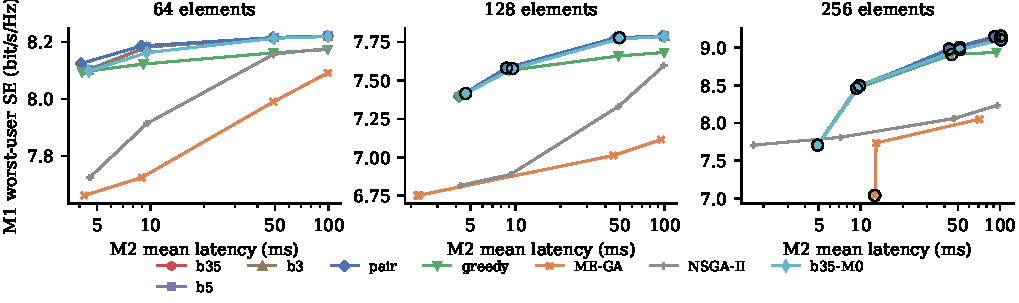
\includegraphics[width=\textwidth]{figures/headline.pdf}

\caption{Sealed test: M1 against M2 at the 5/10/50/100\,ms budgets (M3), one panel per array size. Open black circles mark cells excluded by the 0.5\% miss rule.}\label{fig:headline}
\end{figure}

\begin{table}[t]
\centering
\caption{Pre-registered contrasts at every budget, sealed test: mean difference (bit/s/Hz) and verdict (S supported, ns not supported, ex excluded by the miss rule, nt not testable). 50\,ms is confirmatory.}\label{tab:contrasts}
\scriptsize\setlength{\tabcolsep}{3pt}
\begin{tabular}{@{}ll|rrrr@{}}
\toprule
Contrast & $N$ & 5\,ms & 10\,ms & 50\,ms & 100\,ms\\
\midrule
H1 \bts{}$-$\duet{} & 64 & $-$0.0214 ns & $-$0.0043 ns & +0.0006 ns & +0.0010 S\\
 & 128 & +0.0225 S & +0.0025 ex & $-$0.0004 ns & +0.0004 ns\\
 & 256 & +0.0000 ex & +0.0365 ex & +0.0230 ex & +0.0098 ex\\
H2 \bts{}$-$ME-GA & 64 & +0.4415 S & +0.4571 S & +0.2258 S & +0.1295 S\\
 & 128 & +0.6661 S & +0.8308 S & +0.7662 S & +0.6744 S\\
 & 256 & +0.6688 nt & +1.4587 nt & +1.2700 ex & +1.1035 ex\\
H5 \bts{}$-$NSGA-II & 64 & +0.3772 S & +0.2679 S & +0.0586 S & +0.0441 S\\
 & 128 & +0.6000 S & +0.6954 S & +0.4459 S & +0.1947 S\\
 & 256 & +0.0000 ex & +0.6865 ex & +0.9460 ex & +0.9182 ex\\
\bottomrule
\end{tabular}
\end{table}

\textbf{Evolutionary baselines (H2, H5).} For 64 and 128 elements, both contrasts are supported at every budget (Table~\ref{tab:contrasts}). At 50\,ms, \bts{} exceeds ME-GA by +0.2258 [+0.1283, +0.3315] and +0.7662 [+0.4269, +1.1919]\,bit/s/Hz and NSGA-II by +0.0586 [+0.0275, +0.1091] and +0.4459 [+0.2535, +0.6919]\,bit/s/Hz (64 and 128 elements; Bonferroni-corrected intervals), and it outperforms both baselines on all 18 test trajectories at 64 elements. Plain \duet{} attains the same level (Table~\ref{tab:headline}). Within 50\,ms, \duet{} evaluates 62--445 times more candidates than the evolutionary baselines (M3 in Table~\ref{tab:headline}).

\textbf{Pair moves and the extensions of \bts{} (H1).} \duet{} exceeds single-flip search by +0.0534 [+0.0332, +0.0748] and +0.1188 [+0.0758, +0.1734]\,bit/s/Hz at 50\,ms (descriptive 95\% intervals). H1 is not supported at 50\,ms (+0.0006 [$-$0.0002, +0.0016] at 64 and $-$0.0004 [$-$0.0019, +0.0006] at 128 elements). At other budgets it is supported only in two cells and lies below zero for 64 elements at 5 and 10\,ms (Table~\ref{tab:contrasts}). At 64 elements and 50\,ms, \bts{} $-$ \duetD{} is +0.0011 [+0.0006, +0.0016] and \bts{} $-$ \duetE{} is $-$0.0002 [$-$0.0009, +0.0004].

\textbf{Shortlist and latency (M2).} \bts{}-SL evaluates fewer candidates than \bts{} (52,722 against 72,367 at 64 elements and 50\,ms) and remains slightly below it in M1 at 64 and 128 elements; its selector adds 6.36\,ms per call. All anytime methods consume nearly the entire budget (mean latency of \duet{} at 50\,ms: 48.90 and 46.96\,ms).

\textbf{256 elements.} The \duet{}-family methods exceed the deadline: \bts{} misses 55.31\% and 65.90\% of runs at 50 and 100\,ms, and \duet{} misses 0.62--3.78\% across 5--100\,ms, above the 0.5\% threshold; ME-GA misses all runs at 5 and 10\,ms owing to its initialisation cost. All 256-element contrasts are consequently excluded or not testable (Table~\ref{tab:contrasts}); Sect.~\ref{sec:discussion} analyses the cause.

\subsection{Cross-City Generalisation}\label{sec:crosscity}
To assess external validity without retuning, 48~trajectories (12~check, 36~sealed test) were generated for each of two further European cities, Maastricht and Utrecht, under the Rotterdam placement rules and subjected to the same pre-declared data checks (Table~\ref{tab:cities}). Both cities pass every data check at all array sizes, including the leverage check that the surface can materially change the worst-user rate. Following the Rotterdam deadline analysis, the cross-city evaluation covers 64 and 128 elements, with 72~sealed trajectories (1,152~frames).

\begin{table}[t]
\centering
\caption{GeoRIS-Bench cities used in this paper and their data checks. $L_2$: median worst-user gain (bit/s/Hz) of a long offline search over the all-OFF state on the check split.}\label{tab:cities}
\resizebox{\linewidth}{!}{%
\setlength{\tabcolsep}{4pt}
\begin{tabular}{@{}lccccccc@{}}
\toprule
City & Role & Split (tr/v/te or ch/te) & Size (MB) & Geom.\ agree. & $L_2$ med.\ ($64/128/256$) & Ready arrays & Status \\
\midrule
Rotterdam & development & 83/18/18 (+1 repl.) & --- & 99.28\% & 0.302/0.418/0.782 & 64/128/256 & PASS \\
Maastricht & held-out & 12/36 & 1213.9 & 99.95\% & 0.266/0.241/0.347 & 64/128/256 & PASS \\
Utrecht & held-out & 12/36 & 1212.0 & 99.56\% & 0.130/0.417/0.293 & 64/128/256 & PASS \\
\bottomrule
\end{tabular}%
}
\raggedright{\scriptsize Pre-declared leverage threshold: $L_2\ge0.05/0.07/0.14$ at 64/128/256 elements.}
\vspace{-6pt}
\end{table}

Table~\ref{tab:crosscity} reports the two-city pool ($N=72$; no flagged frames). At 64 elements and 50\,ms, all five contrasts pass: \bts{} $-$ \duet{} is +0.0004 [+0.0001, +0.0009] (42/28/2 wins/losses/ties), and \bts{} outperforms ME-GA (+0.1379) and NSGA-II (+0.0645) on all 72 trajectories; at 10\,ms, the H1 interval lies below zero. At 128 elements and 50\,ms, \duet{} incurs no deadline misses and passes C6 (+0.1998) and C7 (+0.3197) on all 72 trajectories, whereas \bts{} is excluded by a 3.59\% miss rate.

\begin{table}[t]
\centering
\caption{Cross-city benchmark on two held-out cities (pool $N=72$; per-city $N=36$ at $50$\,ms; 99\% Bonferroni CIs for family~5, 95\% CI for descriptive \duet{}$-$\texttt{greedy}).}\label{tab:crosscity}
\resizebox{\linewidth}{!}{%
\setlength{\tabcolsep}{3.5pt}
\begin{tabular}{@{}llcccccc@{}}
\toprule
Array & Subset / Budget & \texttt{greedy} / \duet{} / \bts{} M1 & Miss\% (\duet{}/\bts{}) & $H_1$ (\bts{}$-$\duet{}) & $H_5$ (\bts{}$-$NSGA-II) & $C_6$ (\duet{}$-$NSGA-II) & \duet{}$-$\texttt{greedy} \\
\midrule
$64$ & Pool 10\,ms & 5.3714 / 5.4067 / 5.4034 & 0.00/0.00 & $-$0.0032 [ns, $<0$] & +0.1672 [S] & +0.1704 [S] & +0.0353 [+0.0229, +0.0499] \\
$64$ & Pool 50\,ms & 5.3900 / 5.4191 / 5.4195 & 0.00/0.00 & +0.0004 [S] & +0.0645 [S] & +0.0641 [S] & +0.0290 [+0.0188, +0.0408] \\
$128$ & Pool 10\,ms & 5.9109 / 5.9116 / 5.9146 & 1.15/1.92 & +0.0030 [ex] & +0.2578 [ex] & +0.2549 [ex] & +0.0007 [$-$0.0081, +0.0065] \\
$128$ & Pool 50\,ms & 5.9578 / 5.9898 / 5.9901 & 0.00/3.59 & +0.0002 [ex] & +0.2001 [ex] & +0.1998 [S] & +0.0321 [+0.0180, +0.0491] \\
\midrule
$64$ & Maastricht 50\,ms & 3.4794 / 3.4980 / 3.4982 & 0.00/0.00 & +0.0001 [ns] & +0.0313 [S] & +0.0312 [S] & 33/2/1 wins \\
$64$ & Utrecht 50\,ms & 7.3007 / 7.3401 / 7.3408 & 0.00/0.00 & +0.0007 [S] & +0.0977 [S] & +0.0970 [S] & 36/0/0 wins \\
$128$ & Maastricht 50\,ms & 4.3236 / 4.3341 / 4.3342 & 0.00/1.27 & +0.0001 [ex] & +0.0975 [ex] & +0.0974 [S] & 36/0/0 wins \\
$128$ & Utrecht 50\,ms & 7.5919 / 7.6456 / 7.6459 & 0.00/5.90 & +0.0003 [ex] & +0.3026 [ex] & +0.3023 [S] & 34/2/0 wins \\
\bottomrule
\end{tabular}%
}
\vspace{-6pt}
\end{table}

%======================================================================
\section{Discussion}\label{sec:discussion}
%======================================================================
\textbf{Sources of the advantage over evolutionary search.} Under a fixed deadline, solution quality is governed by the number of informative candidates a method can evaluate. Once $L$ and $R$ are available, a pair candidate costs a few complex multiply--adds, whereas an evolutionary offspring differs from its parents in many bits and requires a solve or a rank-$m$ update (Fig.~\ref{fig:workflow}); this accounts for the 62--445-fold difference in evaluations. ME-GA's memory~\cite{zardi2024memory} is designed to track a channel over many generations, but at 128 elements and 50\,ms it completes approximately two generations of 100 individuals, which leaves its adaptive operators little opportunity to act.

\textbf{Pair versus single-flip moves.} Prior RIS search is limited to single-flip (coordinate) descent~\cite{hammami2026statistical}. Exact pair moves add 0.05--0.12\,bit/s/Hz over single-flip search on Rotterdam and approximately 0.03\,bit/s/Hz on the held-out cities, extending to a non-quadratic coupled objective the observation from binary quadratic programming that larger neighbourhoods escape 1-opt optima~\cite{merz2002bqp}. The restart and recombination rules of \bts{}, standard in memetic search~\cite{lourenco2010ils,merz2004memetic}, yield no measurable improvement here and incur more deadline misses at 128 elements; plain \duet{} is therefore the recommended controller.

\textbf{Exhaustive neighbourhoods under hard deadlines: an open problem.} The 256-element results expose a limitation that is inherent to exhaustive neighbourhoods rather than specific to one implementation. A pair scan is an indivisible unit of work whose size grows quadratically, from 2,016 candidates at 64 elements to 32,640 at 256, while the deadline remains fixed. The deadline check of the \duet{} family reserves a fixed time that does not scale with $N$; at 256 elements this reserve is shorter than one scan, so scans admitted close to the deadline overrun it. Descriptively, the \duet{} family still reaches 8.982--9.005\,bit/s/Hz at 50\,ms, against 7.735 for ME-GA and 8.059 for NSGA-II, but at a mean latency of up to 51.36\,ms, i.e.\ beyond the deadline. At this scale the obstacle is therefore deadline compliance rather than solution quality. How to make exact neighbourhood search interruptible, through scan-time-aware admission, partial scans ordered by predicted gain, or learned pair selection, remains open for real-time control of large coupled surfaces.

\textbf{Limitations.} The evidence is obtained in simulation only, from three European cities whose scenes include LoD2 buildings and terrain but no vegetation, vehicles or street furniture, as is common in ray-traced RIS studies~\cite{peng2025risnet,alkhateeb2019deepmimo,hoydis2023sionna}. Because all methods are compared on identical per-frame channels~\cite{glasserman1992crn}, such simplifications are expected to affect absolute gains, which constitute upper bounds in the presence of foliage loss~\cite{itu2021p833,alnuaimi1998vegetation}, more than the ranking of methods. ME-GA is a reimplementation from its published specification (1-bit elements, fixed precoder, 24 documented gaps), so H2 compares against the specification rather than against published results. Finally, the surface is modelled as perfectly conducting thin wires without substrate or switch parasitics, the precoder is fixed at the all-OFF channel, and perfect channel knowledge is assumed.

%======================================================================
\section{Conclusion}
%======================================================================
This paper presented \duet{}, a deadline-bounded pairwise search that evaluates every single and pair flip of a coupled 1-bit RIS through rank-one and rank-two network updates. Under a hard CPU deadline, it evaluates one to two orders of magnitude more candidates than ME-GA and NSGA-II and achieves higher worst-user rates at 64 and 128 elements on the sealed Rotterdam test split, and these gains transfer without retuning to two unseen cities. Restart densities and elite recombination provide no measurable benefit over plain \duet{}. At 256 elements, a single exhaustive scan no longer fits within the deadline, which identifies interruptible, gain-ordered neighbourhood search as the principal direction for future work, together with validation on measured RIS channels~\cite{tewes2023comprehensive,piana2026brisc}.

\subsubsection*{Data and Code Availability.} Dataset: \url{https://doi.org/10.17632/td3w4cwbg5.1}; dataset code, \duet{} and baselines: \url{https://github.com/ElFariss/GeoRIS-Bench}; experiment scripts, analysis plans and run records: \url{https://github.com/ElFariss/GeoRIS-Physics}.

\subsubsection*{Disclosure of Interests.} The authors have no competing interests to declare that are relevant to the content of this article.

\bibliographystyle{splncs04}
\bibliography{references}
\end{document}
